\documentclass[10pt]{article}  

%%%%%%%% PREÁMBULO %%%%%%%%%%%%
\title{Plantilla para prácticas de UGR}
\usepackage[spanish]{babel} %Indica que escribiermos en español
\usepackage[utf8]{inputenc} %Indica qué codificación se está usando ISO-8859-1(latin1)  o utf8  
\usepackage{amsmath} % Comandos extras para matemáticas (cajas para ecuaciones,
% etc)
\usepackage{amssymb} % Simbolos matematicos (por lo tanto)
\usepackage{graphicx} % Incluir imágenes en LaTeX
\usepackage{color} % Para colorear texto
\usepackage{subfigure} % subfiguras
\usepackage[dvipsnames]{xcolor}
\usepackage{float} %Podemos usar el especificador [H] en las figuras para que se
% queden donde queramos
\usepackage{capt-of} % Permite usar etiquetas fuera de elementos flotantes
% (etiquetas de figuras)
\usepackage{sidecap} % Para poner el texto de las imágenes al lado
	\sidecaptionvpos{figure}{c} % Para que el texto se alinie al centro vertical
\usepackage{caption} % Para poder quitar numeracion de figuras
\usepackage{commath} % funcionalidades extras para diferenciales, integrales,
% etc (\od, \dif, etc)
\usepackage{cancel} % para cancelar expresiones (\cancelto{0}{x})

\graphicspath{{/Users/jesusgarciamanday/Documents/Master/IC/Practicas/Practica1/p1/Imagenes/}}

\usepackage{anysize} 					% Para personalizar el ancho de  los márgenes
\marginsize{2cm}{2cm}{2cm}{2cm} % Izquierda, derecha, arriba, abajo

\usepackage{appendix}
\renewcommand{\appendixname}{Apéndices}
\renewcommand{\appendixtocname}{Apéndices}
\renewcommand{\appendixpagename}{Apéndices} 

% Para que las referencias sean hipervínculos a las figuras o ecuaciones y
% aparezcan en color
\usepackage[colorlinks=true,plainpages=true,citecolor=blue,linkcolor=blue]{hyperref}
%\usepackage{hyperref} 
% Para agregar encabezado y pie de página
\usepackage{fancyhdr} 
\pagestyle{fancy}
\fancyhf{}
\fancyhead[L]{\footnotesize UGR} %encabezado izquierda
\fancyhead[R]{\footnotesize CCIA}   % dereecha
\fancyfoot[R]{\footnotesize Inteligencia Computacional }  % Pie derecha
\fancyfoot[C]{\thepage}  % centro
\fancyfoot[L]{\footnotesize Master en Ingenier\'ia Inform\'atica }  %izquierda
\renewcommand{\footrulewidth}{0.4pt}


\usepackage{listings} % Para usar código fuente
\definecolor{dkgreen}{rgb}{0,0.6,0} % Definimos colores para usar en el código
\definecolor{gray}{rgb}{0.5,0.5,0.5} 
% configuración para el lenguaje que queramos utilizar
\lstset{language=Matlab,
   keywords={break,case,catch,continue,else,elseif,end,for,function,
      global,if,otherwise,persistent,return,switch,try,while},
   basicstyle=\ttfamily,
   keywordstyle=\color{blue},
   commentstyle=\color{red},
   stringstyle=\color{dkgreen},
   numbers=left,
   numberstyle=\tiny\color{gray},
   stepnumber=1,
   numbersep=10pt,
   backgroundcolor=\color{white},
   tabsize=4,
   showspaces=false,
   showstringspaces=false}

\newcommand{\sen}{\operatorname{\sen}}	% Definimos el comando \sen para el seno
%en español

\title{Inteligencia Computacional}

%%%%%%%% TERMINA PREÁMBULO %%%%%%%%%%%%

\begin{document}

%%%%%%%%%%%%%%%%%%%%%%%%%%%%%%%%%% PORTADA %%%%%%%%%%%%%%%%%%%%%%%%%%%%%%%%%%%%%%%%%%%%
																					%%%
\begin{center}																		%%%
\newcommand{\HRule}{\rule{\linewidth}{0.5mm}}									%%%\left
 																					%%%
\begin{minipage}{0.48\textwidth} \begin{flushleft}
%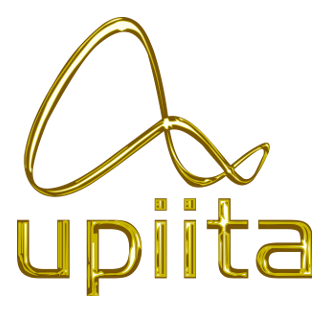
\includegraphics[scale = 0.63]{Imagenes/logo_upiita}
\end{flushleft}\end{minipage}
\begin{minipage}{0.48\textwidth} \begin{flushright}
%
\includegraphics[scale = 0.35]{Imagenes/IPN}
\end{flushright}\end{minipage}

													 								%%%
\vspace*{-1.5cm}								%%%
																					%%%	
\textsc{\huge Universidad de\\ \vspace{5px} Granada}\\[1.5cm]	

\textsc{\LARGE Master Profesional en Ingenier\'ia Inform\'atica }\\[1.5cm]													%%%

\begin{minipage}{0.9\textwidth} 
\begin{center}																					%%%
\textsc{\LARGE Pr\'actica 1}
\end{center}
\end{minipage}\\[0.5cm]
%%%
    																				%%%
 			\vspace*{1cm}																		%%%
																					%%%
\HRule \\[0.4cm]																	%%%
{ \huge \bfseries MNIST}\\[0.4cm]	%%%
 																					%%%
\HRule \\[1.5cm]																	%%%
 																				%%%
																					%%%
\begin{minipage}{0.46\textwidth}													%%%
\begin{flushleft} \large															%%%
\emph{Autor:}\\	
Manuel Jes\'us Garc\'ia Manday (nickter@correo.ugr.es)\\
%%%
			%\vspace*{2cm}	
            													%%%
										 						%%%
\end{flushleft}																		%%%
\end{minipage}		
																%%%
\begin{minipage}{0.52\textwidth}		
\vspace{-0.6cm}											%%%
\begin{flushright} \large															%%%
													%%%
\end{flushright}																	%%%
\end{minipage}	
\vspace*{1cm}
%\begin{flushleft}
 	
%\end{flushleft}
%%%
 		\flushleft{\textbf{\Large Master en Ingenier\'ia Inform\'atica}	}\\																		%%%
\vspace{2cm} 																				
\begin{center}																					
%{\large 20 de abril de 2017}																	%%%
 			\end{center}												  						
\end{center}							 											
																					
\newpage																		
%%%%%%%%%%%%%%%%%%%% TERMINA PORTADA %%%%%%%%%%%%%%%%%%%%%%%%%%%%%%%%

\tableofcontents 

\newpage



\section{Introducción.} 
Para la resolución de esta práctica se han empleado tres tipos de modelos diferentes de redes neuronales artificiales para intentar resolver el problema de reconocimiento de dígitos manuscritos que proporciona la base de datos MNIST. Para cada modelo de red se han realizado varias pruebas, variando los parámetros de cada uno de ellos en función de los resultados obtenidos. \\

En siguientes apartados se detallará todo el proceso realizado así como los diferentes resultados conseguidos con cada prueba. 



\section{Entorno de trabajo.} 
Se ha definido un entorno de trabajo donde se desarrollarán las implementaciones de los diferentes modelos redes así como sus pruebas. Dicho entorno está basado en \textbf{Python} \footnote{Disponible en el sitio web de Python (https://www.python.org)} en su versión \textbf{3.5}. Para la implementación de los modelos de redes se va emplear la librería \textbf{Keras} \footnote{Disponible en el sitiio web de Keras (https://keras.io)} en su versión \textbf{2.0.2}, la cual a su vez se apoya en la versión \textbf{1.0.1} de la librería \textbf{Tensorflow} \footnote{Disponible en el sitio web de Tensorflow (https://www.tensorflow.org)}. Mediante esta API definiremos los tres modelos de redes neuronales que serán entrenados y testeados con sus respectivos conjunto de datos. \\

Keras es una API de alto nivel para la creación de redes neuronales escrita en Python que se ejecuta por encima de otras librerías como la mencionada Tensorflow, \textbf{CNTK} \footnote{Disponible en el girhub de CNTK (https://github.com/Microsoft/cntk)} o \textbf{Theano} \footnote{Disponible en el sitio web de Theano (http://www.deeplearning.net/software/theano/)}. Soporta ambos tipos de redes neuronales, convolutivas y recurrentes además de su combinación. Se puede ejecutar tanto en CPU como en GPU. \\

Tensorflow es una librería de código abierto usada para computación numérica usando gráficos de flujos de datos. Posee una arquitectura flexible que permite realizar aplicaciones de cómputo en una o mas CPUs o GPUs en un ordenador personal, servidor o dispositivo móvil. \\

CNTK (Computational Network Toolkit) actualmente conocido como \textbf{The Microsoft Cognitive Toolkit} es el motor de intelegencia artificial de Microsoft a través del cual se proporcionan librerías para trabajar con redes neuronales. \\

Theano es una librería escrita en Python que permite definir, optimizar y evaluar expresiones matemáticas envueltas en arrays multidimensionales de manera eficiente. Entre sus propiedades se puede destacar la fuerte integración que tiene con la librería \textbf{NumPy} \footnote{Disponible en el sitio web de NumPy (http://www.numpy.org)}, el uso transparente de la GPU, etc. \\



\section{Modelos de redes neuronales} 
Como se ha mencionado anteriormente, son tres los diferentes tipos de modelo de red neuronal los que se han implementado. Una red neuronal simple con una capa de entrada y una capa de salida, una red neuroal multicapa con una capa oculta, y una red neuronal convolutiva con diferentes niveles de capas. A estos tipos de modelo de red neuronal se le han ido aplicando variaciones en sus parámetros para ajustar los resultados que se han ido obteniendo como se demostrará en el actual apartado. \\

Se ha definido un script base en python en el que se apoyarán todas las implementaciones y pruebas de los diferentes modelos de red. Este script obtiene los conjuntos de imágenes y etiquetas de MNIST, tanto de entrenamiento como de prueba. Las imágenes obtenidas, que tienen sus valores de escala de grises representados en estructuras de array de dos dimensiones, son convertidos a un array de una sola dimensión. Estos valores a su vez son normalizados de 0 a 1. Del mismo modo las etiquetas son también obtenidas y tratadas para el entrenamiento y testeo de la red neuronal. \\

\begin{figure}[H]
	\begin{center}
 		\includegraphics[width = 0.75\textwidth]{p1-img1}
 		\captionof{figure}{\label{fig:IPN}Descarga de imágenes de MNIST y paso a array de una dimensión.} 
	\end{center} 
\end{figure}

El primer modelo de red neuronal implementado es un modelo muy simple que consta de una capa de entrada y una capa de salida. La capa de entrada esta formada por 784 neuronas, el equivalente al número de pixeles de una imagen (28x28), las neuronas de una capa de entrada no son de procesamiento a diferencia del resto. En la capa de salida se definen 10 neuronas, el equivalente al número de clases que una imagen puede tomar, las cuales tienen una función de activación \textit{softmax}. En la siguiente figura se puede ver la implementación de este modelo de red neuronal. \\

\begin{figure}[H]
	\begin{center}
 		\includegraphics[width = 1.00\textwidth]{p1-img2}
 		\captionof{figure}{\label{fig:IPN}Modelo de red neuronal con una capa de entrada y una capa de salida.} 
	\end{center} 
\end{figure}

Una vez definido el modelo de red pasamos a entrenarlo y posteriormente a testearlo. Para el entrenamiento de los modelos de red se utilizará el conjunto de datos de MNIST destinado a ello, el cual se compone de 60.000 imágenes de dígitos manuscritos. Se establecerán 10 épocas para el entrenamiento y un tamaño de batch de 200. El conjunto de imágenes de test para la red lo forman 10.000 imágenes. \\

\begin{figure}[H]
	\begin{center}
 		\includegraphics[width = 1.00\textwidth]{p1-img3}
 		\captionof{figure}{\label{fig:IPN}Entrenamiento de red neuronal simple.} 
	\end{center} 
\end{figure}

\begin{figure}[H]
	\begin{center}
 		\includegraphics[width = 1.00\textwidth]{p1-img5}
 		\captionof{figure}{\label{fig:IPN}Prueba de red neuronal simple.} 
	\end{center} 
\end{figure}

\begin{figure}[H]
	\begin{center}
 		\includegraphics[width = 1.00\textwidth]{p1-img4}
 		\captionof{figure}{\label{fig:IPN}Resultados red neuronal simple.} 
	\end{center} 
\end{figure}

Se puede ver en la \textbf{Figura 4} como se ha obtenido un resultado del \textbf{1.83\%} de error sobre el conjunto de prueba en un tiempo total de 59 segundos. No es una buena solución, por lo que vamos a probar a definir otro modelo de red neuronal para mejorar esos resultados. \\

Siguiendo la línea del modelo anterior definido, lo que se propone en esta solución es añadir nuevas capas ocultas para mejorar el proceso de aprendizaje ya que con un modelo de red neuronal simple los perceptrones no son capaces de extraer tanto nivel de características. A este tipo de redes se les conoce como redes neuronales multicapas. El modelo de red definido tiene la estructura que muestra la siguiente figura. \\

\begin{figure}[H]
	\begin{center}
 		\includegraphics[width = 1.00\textwidth]{p1-img6}
 		\captionof{figure}{\label{fig:IPN}Red neuronal multicapa.} 
	\end{center} 
\end{figure}

Como se puede apreciar en la imagen, el modelo de red mantiene el mismo número de neuronas en las capas de entrada y de salida que el modelo anterior. La capa oculta de este modelo se compone una única capa con la mitad de neuronas que la capa de entrada. Tras entrenar la red con los datos pertinentes, el testeo de la misma devolvió los siguientes resultados. \\

\begin{figure}[H]
	\begin{center}
 		\includegraphics[width = 1.00\textwidth]{p1-img7}
 		\captionof{figure}{\label{fig:IPN}Resultado prueba red neuronal multicapa.} 
	\end{center} 
\end{figure}

Podemos observar como el resultado en la precisión de acierto ha mejorado con respecto al modelo de red anterior de un \textbf{1.82\%} a un \textbf{1.58\%}. Una mejora evidente debida a la inclusión de la capa oculta en el modelo. \\

Aunque el porcentaje de error ha disminuido con la propuesta de este nuevo modelo, con algunas variaciones podemos seguir intentando reducirlo más. Vamos a probar a modificar el número de neuronas de la única capa que hay dentro de la capa oculta para observar si los resultados son favorables. Para ellos definimos este nuevo modelo de red neuronal. \\

\begin{figure}[H]
	\begin{center}
 		\includegraphics[width = 1.00\textwidth]{p1-img8}
 		\captionof{figure}{\label{fig:IPN}Red neuronal multicapa (ii).} 
	\end{center} 
\end{figure}

Este nuevo modelo mantiene el mismo número de capas que el anterior, con la modificación del número de neuronas de la capa oculta que pasa a tener el mismo que la capa de entrada. Con la nueva red neuronal definida pasamos a entrenarla y testearla para observar su comportamiento. \\

\begin{figure}[H]
	\begin{center}
 		\includegraphics[width = 1.00\textwidth]{p1-img9}
 		\captionof{figure}{\label{fig:IPN}Resultados red neuronal multicapa (ii).} 
	\end{center} 
\end{figure}

La imagen de la \textbf{Figura 9} nos muestra en el resultado como ha aumentado el porcentaje de error en el acierto, lo que nos marca que el modelo de red definido no mejora al anterior. Probaremos esta vez a reducir en cuatro veces el número de neuronas de la capa oculta y ver que resultados arroja una vez que esta haya sido entrenada. \\

\begin{figure}[H]
	\begin{center}
 		\includegraphics[width = 1.00\textwidth]{p1-img10}
 		\captionof{figure}{\label{fig:IPN}Red neuronal multicapa (iii).} 
	\end{center} 
\end{figure}

\begin{figure}[H]
	\begin{center}
 		\includegraphics[width = 1.00\textwidth]{p1-img11}
 		\captionof{figure}{\label{fig:IPN}Resultados red neuronal multicapa (iii).} 
	\end{center} 
\end{figure}

Vemos que el resultado lanzado por el nuevo modelo de red no mejora tampoco el hasta ahora mejor resultado obtenido con el primer modelo de red neuronal multicapa. El porcentaje de error en el acierto empeora al obtenido con el anterior modelo de red, por lo que el decrementar tanto el número de neuronas en la capa oculta no aporta buenos resultados. \\

Siguiendo con este tipo de red neuronal, vamos ahora a implementar un nuevo modelo en el que se va a introducir una nueva capa en la capa oculta. De este modo la capa oculta estará compuesta por dos capas en lugar de una sola como en el ejemplo anterior. Estas dos capas en principio van a tener el mismo número de neuronas, el correspondiente a la mitad de las que posee la capa de entrada, es decir, tanto la primera capa como la segunda de la capa oculta tendrán la mitad de neuronas que la capa de entrada. \\

\begin{figure}[H]
	\begin{center}
 		\includegraphics[width = 1.00\textwidth]{p1-img12}
 		\captionof{figure}{\label{fig:IPN}Red neuronal multicapa (iv).} 
	\end{center} 
\end{figure}

\begin{figure}[H]
	\begin{center}
 		\includegraphics[width = 1.00\textwidth]{p1-img13}
 		\captionof{figure}{\label{fig:IPN}Resultados red neuronal multicapa (iv).} 
	\end{center} 
\end{figure}

Analizando el resultado obtenido con este nuevo modelo de red se puede observar como seguimos sin mejorar el mejor porcentaje de error conseguido hasta ahora de \textbf{1.58\%}. Vamos a variar los parámetros del número de neuronas de las capas dentro de la capa oculta para analizar el comportamiento de los resultados que se obtengan. \\

Se ha definido un primer modelo de red en base al anterior en el que esta vez la primera capa oculta mantiene el mismo número de neuronas que la capa de entrada, mientras que la segunda capa oculta continua manteniendo la mitad. \\

\begin{figure}[H]
	\begin{center}
 		\includegraphics[width = 1.00\textwidth]{p1-img14}
 		\captionof{figure}{\label{fig:IPN}Red neuronal multicapa (v).} 
	\end{center} 
\end{figure}

\begin{figure}[H]
	\begin{center}
 		\includegraphics[width = 1.00\textwidth]{p1-img15}
 		\captionof{figure}{\label{fig:IPN}Resultados red neuronal multicapa (v).} 
	\end{center} 
\end{figure}

No se han mejorado los resultados con este nuevo modelo viendo su \textbf{1.78\%} de error en el acierto, por lo que vamos a modificar los parámetros de este variando el número de neuronas de las capas ocultas. En esta ocasión la primera capa oculta tendrá la mitad de neuronas que la capa de entrada, mientras que la segunda capa oculta se compondrá del mismo número de neuronas que las que tiene que la capa de entrada. \\

\begin{figure}[H]
	\begin{center}
 		\includegraphics[width = 1.00\textwidth]{p1-img16}
 		\captionof{figure}{\label{fig:IPN}Red neuronal multicapa (vi).} 
	\end{center} 
\end{figure}

\begin{figure}[H]
	\begin{center}
 		\includegraphics[width = 1.00\textwidth]{p1-img17}
 		\captionof{figure}{\label{fig:IPN}Resultados red neuronal multicapa (vi).} 
	\end{center} 
\end{figure}

Se puede apreciar como los resultados que estamos obteniendo no tienden a mejorar el que hasta ahora es el más óptimo. En esta ocasión con el modelo anterior se ha conseguido un \textbf{1.80\%} en segundos, lo que hace seguir en la misma línea que el anterior. \\

Mateniendo esta misma línea de modelo de red, vamos a optar por introducir otra capa oculta más para analizar el resultado que podemos obtener con esta nueva opción. Para ello, partiendo del modelo de red en el que hasta ahora se han estado basando todos los demás, añadiremos una nueva capa oculta. Se mantendrá el número de neuronas para las dos primeras capas ocultas, es decir, el mismo que la capa de entrada para la primera capa oculta y la mitad de las neuronas para la segunda capa oculta. Esta tercera capa estará compuesta por el mismo número de neuronas que la segunda. En la siguiente imagen se puede ver el nuevo modelo de red definido. \\

\begin{figure}[H]
	\begin{center}
 		\includegraphics[width = 1.00\textwidth]{p1-img18}
 		\captionof{figure}{\label{fig:IPN}Red neuronal multicapa (vii).} 
	\end{center} 
\end{figure}

\begin{figure}[H]
	\begin{center}
 		\includegraphics[width = 1.00\textwidth]{p1-img19}
 		\captionof{figure}{\label{fig:IPN}Resultados red neuronal multicapa (vii).} 
	\end{center} 
\end{figure}

Una vez entrenada y testeada esta nueva red se puede observar como sigue sin disminuir el error en el acierto con un \textbf{2.02\% } obtenido en esta ocasión, que ha padecido un aumento debido posiblemente al sobre-entremiento de la misma. Este último experimento hace que nos planteemos una nueva alternativa de modelo de red neuronal dando paso a los modelos de redes neuronales convolutivas. \\

Este tipo de modelo de red es característico por las capas de convolución y agrupación que sufren los datos de entrada. La capa de convolución es el primer proceso por el que pasan los datos de entrada. El cometido de este capa es aplicar un filtro de tamaño que oscila entre 3x3 y 5x5 a la matriz de datos de entrada que forma la imagen, y obtener un conjunto de mapas de características de la misma. Con este proceso se obtienen mapas de características que esencialmente es la misma imagen que la de entrada, pero donde cada píxel es mucho mas rico en información ya que contiene información sobre la región en la que se encuentra y no sólo la del propio pixel.  Con la aplicación de esta capa se consigue también reducir el número de conexiones y de parámetros a entrenar en comparación con una red neuronal multicapa.\\

La otra capa que se va aplicar en el nuevo modelo de red neuronal es una capa de agrupación o de \textit{pooling}. Esta capa toma como datos de entrada los mapas de características generados por la capa anterior y agrupa dichas características de varias coordenadas contiguas con alguna función de agrupación como la media o el máximo. La salida de esta capa será los mismos mapas de características que tomó de entrada, pero con el tamaño reducido en función del tipo de agrupamiento que se realice (2 ó 4 suele ser lo normal ya que un factor de agrupamiento mayor puede hacer perder información de características) . \\

En esta tesitura, se ha implementado un modelo de red neuronal convolutiva como el que se muestra en la siguiente imagen, el cual se ha entrenado y testeado siguiendo el mismo proceso que los anteriores para comprobar su nivel de acierto en la clasificación de las imágenes de dígitos manuscritos. La capa de convolución que se aplica en este modelo de red generará 32 mapas de características empleando para ello unos filtros de tamaño 5x5. La segunda capa, de agrupamiento, utilizará un factor (2,2), lo que hará que el tamaño de los array de entrada a esta capa se reduzcan a la mitad a su salida. \\

\begin{figure}[H]
	\begin{center}
 		\includegraphics[width = 1.00\textwidth]{p1-img20}
 		\captionof{figure}{\label{fig:IPN}Red neuronal convolutiva (i).} 
	\end{center} 
\end{figure}

\begin{figure}[H]
	\begin{center}
 		\includegraphics[width = 1.00\textwidth]{p1-img21}
 		\captionof{figure}{\label{fig:IPN}Resultados red neuronal convolutiva (i).} 
	\end{center} 
\end{figure}

Se puede apreciar como el resultado de \textbf{0.96\%} de error en el acierto obtenido ha mejorado notablemente el que hasta ahora era el mejor conseguido de \textbf{1.58\%} ya que incluso ha bajado de 1, lo que nos manifiesta que de las 10000 imágenes de prueba sólo se ha equivocado en 96. En el nuevo modelo de red neuronal convolutiva, ademas de las capas de convolución y agrupación que hacen que las neuronas extraigan mejor información de las caracterísitcas, también se aplican dos procesos que ayudan a agilizar la información de entrada que se presenta a las neuronas de procesamiento. Se emplea un método \textit{dropout} para aleatoriamente establecer a 0 el valor de algunos datos de entrada y evitar de este modo el sobre-entrenamiento. También se aplica un método de \textit{flatten} para representar los datos de entrada en un array de una dimensión en lugar de la representación de dos dimensiones que es como se obtienen. Por último, se agrega una capa de neuronas en la capa oculta que contiene 128 neuronas de procesamiento con una función de activación  \textit{relu}. La capa de salida se mantiene siendo la misma que en el resto de experimentaciones anteriores, es decir, con 10 neuronas correspondientes a los diferentes tipos de clasificación, y una función de activación \textit{softmax}.\\

Viendo las notables mejoras que este modelo de red presenta, se va a definir otro nuevo modelo de red neuronal convolutiva siguiendo la misma línea que el anterior. Tomándo este base, la siguiente propuesta de modelo de red va contener una capa mas de convolución y otra de agrupamiento. Los parámetros de las capas de convolución serán diferentes, generando la primera capa 30 mapas de características usando unos filtros de 5x5, mientras que la segunda capa generará 15 mapas utilizando filtros de tamaño 3x3. Ambas capas emplearán la misma función de activación \textit{relu}. \\

Las dos capas de agrupación tomarán el mismo parámetro (2,2), reduciendo a la mitad el tamaño de los mapas de características que reciben como entrada. También se añadirá una capa más de neuronas con un tamaño de 50 a la que ya existe de 128, ambas con la función \textit{relu} como función de activación. \\

Definida la red, pasamos a entrenarla y probarla para ver su comportamiento. \\

\begin{figure}[H]
	\begin{center}
 		\includegraphics[width = 1.00\textwidth]{p1-img22}
 		\captionof{figure}{\label{fig:IPN}Red neuronal convolutiva (ii).} 
	\end{center} 
\end{figure}

\begin{figure}[H]
	\begin{center}
 		\includegraphics[width = 1.00\textwidth]{p1-img23}
 		\captionof{figure}{\label{fig:IPN}Resultados red neuronal convolutiva (ii).} 
	\end{center} 
\end{figure}


Nuevamente el resultado ha vuelto a mejorar bajando el porcentaje de error en el acierto hasta un \textit{0.73\%} con respecto al anterior, lo que confirma que el aumentar las capas de convolución y agrupamiento así como la de neuronas, hace que estas últimas obtengan unas caraterísticas de mejor calidad. \\

Con el objetivo de seguir mejorando la precisión de acierto de la red neuronal vamos a volver a definir un nuevo modelo de red neuronal convolutiva tomando el anterior y modificando una serie de parámetros. Observando que las mejoras han venido producidas por las capas de convolución y de agrupamiento, se van a modificar los parámetros del primer tipo. A las dos capas de convolución existentes se les va a aumentar el número de mapas de características a generar, siendo 40 en la primera y 20 en la segunda. En ambas se mantendrá tanto el tamaño del filtro como la función de activación como se puede visualizar en las imágenes. \\

\begin{figure}[H]
	\begin{center}
 		\includegraphics[width = 1.00\textwidth]{p1-img24}
 		\captionof{figure}{\label{fig:IPN}Red neuronal convolutiva (iii).} 
	\end{center} 
\end{figure}

\begin{figure}[H]
	\begin{center}
 		\includegraphics[width = 1.00\textwidth]{p1-img25}
 		\captionof{figure}{\label{fig:IPN}Resultados red neuronal convolutiva (iii).} 
	\end{center} 
\end{figure}

Se puede apreciar en las imagenes de arriba como de nuevo el porcentaje de error en el acierto vuelve a disminuir hasta el \textbf{0.67\%} con este nuevo modelo de red neuronal convolutiva como fruto del aumento de los mapas de características a generar en las capas de convolución. \\

Con este nuevo resultado obtenido que mejora a todos los anteriores, vamos a definir un nuevo modelo de red para intentar decrementar algo más el porcentaje de error actual. Tomando el mismo modelo de red neuronal convolutiva con el que hemos obtenido el mejor resultado, es decir, el que se visualiza en la \textbf{Figura 24} vamos a realizar el mismo proceso que antes aumentando el número de mapas producir por las capas de convolución. En esta ocasión, a la primera capa se le asignará 50 mapas de características y 25 a la segunda. El resto de parámetros se mantendrán igual. \\

Se pasará a entrenar y probar el nuevo modelo de red para analizar el resultado. \\

 \begin{figure}[H]
	\begin{center}
 		\includegraphics[width = 1.00\textwidth]{p1-img26}
 		\captionof{figure}{\label{fig:IPN}Red neuronal convolutiva (iv).} 
	\end{center} 
\end{figure}

\begin{figure}[H]
	\begin{center}
 		\includegraphics[width = 1.00\textwidth]{p1-img27}
 		\captionof{figure}{\label{fig:IPN}Resultados red neuronal convolutiva (iv).} 
	\end{center} 
\end{figure}

En esta ocasión el porcentaje de error no ha disminuido sino que ha aumentando hasta un \textbf{0.74\%}. Esto puede ser debido a que al aumentar el número de mapas de características generados por la capa de convolución se haya repetido mucho información de los datos dando lugar a que haya algo de sobre-aprendizaje.\\

Como se ha podido comprobar con las pertinentes experimentaciones realizadas, el modelo de red neuronal convolucional es el que mejor resultado ha obtenido llegando al \textbf{0.67\%} lo que hace que sólo se equivoque en 67 imágenes de las 10000 de prueba. Son varias las conclusiones que se pueden extraer con los resutaldos de la batería de pruebas que se ha realizado con todos los modelos de redes neuronales, pero sin duda el que se realice previamente un proceso de convolución y agrupamiento parece ser clave para que las capas de neuronas reciban con mayor claridad los datos de entradas. También es importante reseñar que en función de los parámetros que se configuren en estas capas se podrá ajustar en mayor o menor medida el resultado del porcentaje de error en el acierto de las imágenes. \\

Es por eso por lo que hay que probar diversas configuraciones hasta encontrar los parámetros óptimos para la correcta clasificación de las imágenes de dígitos manuscritos.\\ \\ \\ \\ \\ \\ \\ \\ \\ \\ \\ \\


\section{Listado de soluciones.}  

En la siguiente tabla se muestran las diferentes soluciones obtenidas:

\begin{table}[htbp]
\begin{center}
\begin{tabular}{|l|l|l|l|l|l|}
\hline
Tipo de red & Capas ocultas (*) & Capas convolución (**) & Capas pooling & \% Error & Tiempo (segundos) \\
\hline \hline
Simple & 0 & - & - & 1.83 & 59 \\ \hline
Multicapa & 1(392) & - & - & 1.58 & 108 \\ \hline
Multicapa & 1(784) & - & - & 1.74 & 125 \\ \hline
Multicapa & 1 (196) & - & - & 1.85 & 78 \\ \hline
Multicapa & 2 (392, 392) & - & - & 1.75 & 115 \\ \hline
Multicapa & 2 (784, 392) & - & - & 1.78 & 162 \\ \hline
Multicapa & 2 (392, 784) & - & - & 1.80 & 133 \\ \hline
Multicapa & 2 (392, 392) & - & - & 2.02 & 111 \\ \hline
Convolutiva & 1 (128) & 1(32) & 1 & 0.96 & 1406 \\ \hline
Convolutiva & 2 (128, 50) & 2(30, 15) & 2 & 0.73 & 1628 \\ \hline
Convolutiva & 2 (128, 50) & 2(40, 20) & 2 & 0.67 & 2328 \\ \hline
Convolutiva & 2 (128, 50) & 2(50, 25) & 2 & 0.74 & 2244 \\ \hline
\end{tabular}
(*) número de neuronas\\
(**) número de mapas\\
\caption{Lista de soluciones.}
\label{tabla:sencilla}
\end{center}
\end{table}

Se puede apreciar como los resultados obtenidos con las redes neuronales convolutivas son los que menor porcentaje de error en el acierto tienen, incrementando considerablemente el tiempo de cómputo. \\ \\ \\


\section{Bibliografía.}  

\url{https://machinelearningmastery.com/tutorial-first-neural-network-python-keras/} \\

\url{http://adventuresinmachinelearning.com/keras-tutorial-cnn-11-lines/} \\

\url{https://elitedatascience.com/keras-tutorial-deep-learning-in-python}\\


\end{document}


